\documentclass[dvipsnames]{article}
\usepackage[utf8]{inputenc}
\usepackage[left=3cm, right=3cm, top=2cm]{geometry}
\title{Dynamic Boundary Conditions}
\author{Silvin Willemsen}
\date{June 2020}

\usepackage{natbib}
\usepackage{graphicx}
\usepackage{appendix}
\usepackage{amsmath}
\usepackage{amsfonts}
\usepackage{amssymb}
\usepackage{subfig}

\usepackage{xcolor}
\def\SBcomment[#1]{\textcolor{red}{#1}}
\def\SWcomment[#1]{\textcolor{blue}{#1}}
\def\SScomment[#1]{\textcolor{green}{#1}}
\def\type[#1]{\textcolor{purple}{#1}}

\begin{document}
\maketitle

\section{Introduction}
This document shows the work done and documentation on dynamic boundary conditions.
 
\section{Explanation}
Let's take the 1D wave equation in discrete time:
\begin{equation}
    \rho A\delta_{tt}u_l^n=T\delta_{xx}u_l^n
\end{equation}
with simply supported boundary conditions such that
\begin{equation}\label{eq:1Dwave}
u_l^n = \delta_{xx}u_l^n = 0 \quad \text{at} \quad l = 0, N.
\end{equation}

Through stability analysis one can arrive at a condition for the grid spacing that needs to be satisfied in order for the implementation to be stable. In this case this is
\begin{equation}\label{eq:stabilityCondition}
    h \geq ck,
\end{equation}
where $c = \sqrt{T/\rho A}$. The closer $h$ is to this condition, the more accurate the scheme will be. 
Consider a string with a wavespeed of $c = 1470$ m/s. With $f_\text{s} = 44100$ we can satisfy condition \eqref{eq:stabilityCondition} with equality $h = 0.333$.

\begin{figure*}[ht!]
    \centering
    \subfloat[String $N=30$.]{\label{fig:echoIde}{ 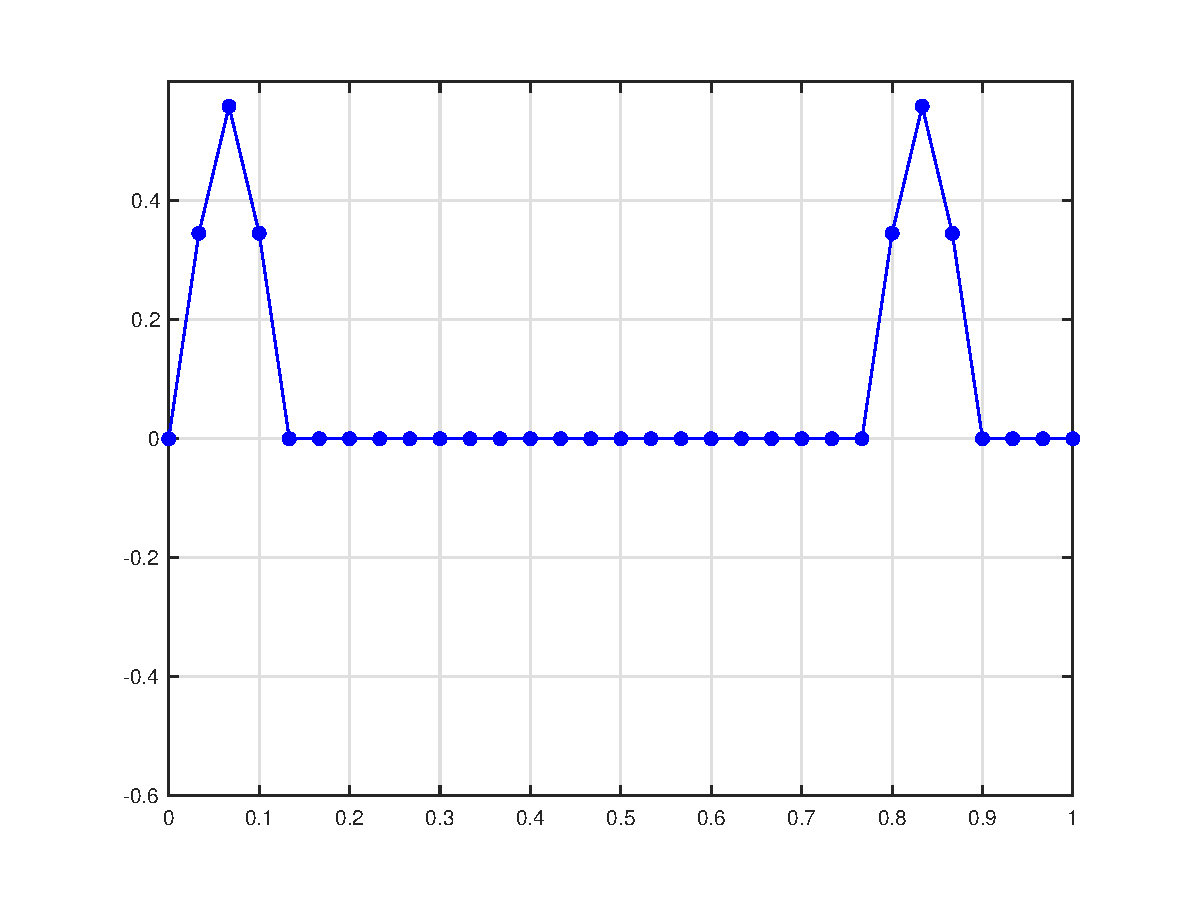
\includegraphics[width=0.33\textwidth]{plot1.eps}}}
    \subfloat[At the left boundary.]{\label{fig:echoHouse}{ 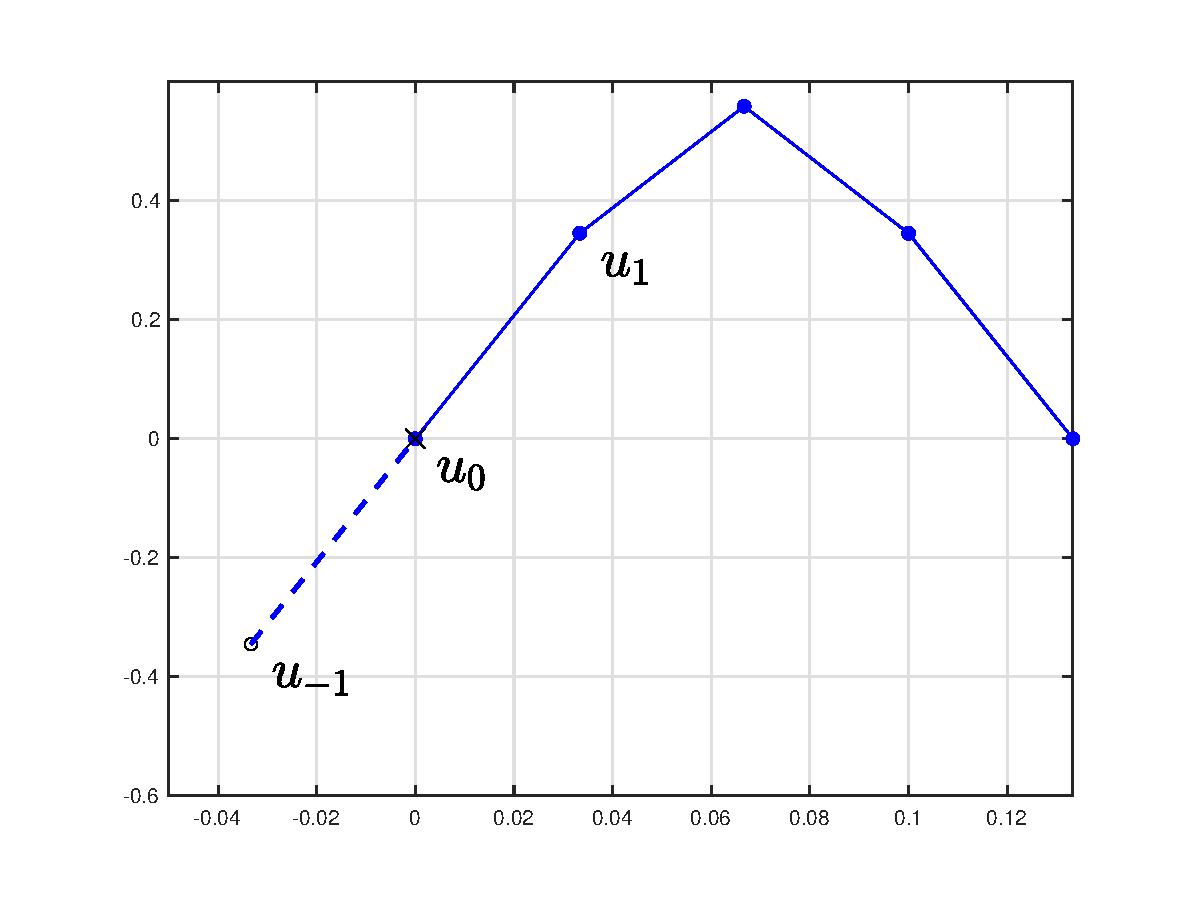
\includegraphics[width=0.33\textwidth]{plot2.eps}}}
    \subfloat[Curvature at the boundary (in this case $u_0$) should be 0.]{\label{fig:echoHad}{ 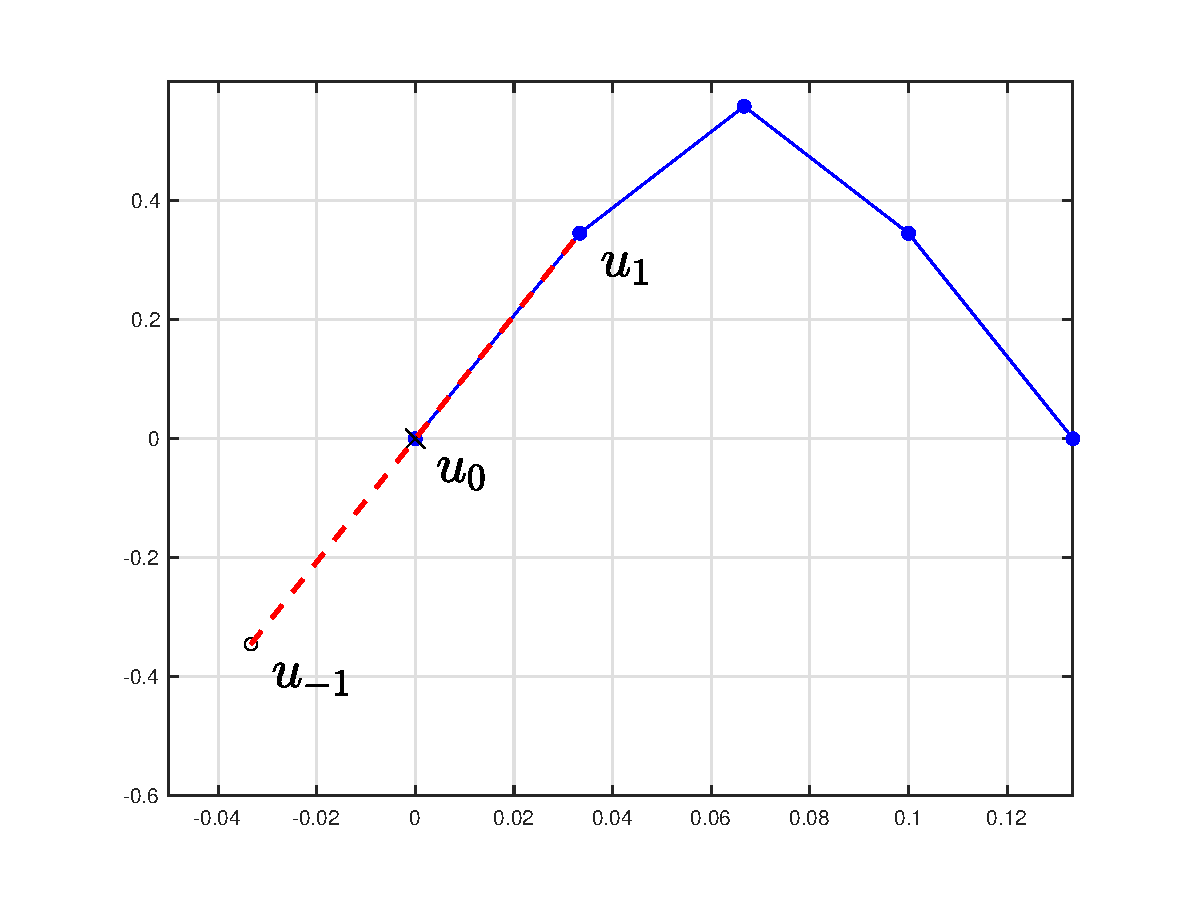
\includegraphics[width=0.33\textwidth]{plot3.eps}}}
\end{figure*}


% \begin{figure}[h]
% \centerline{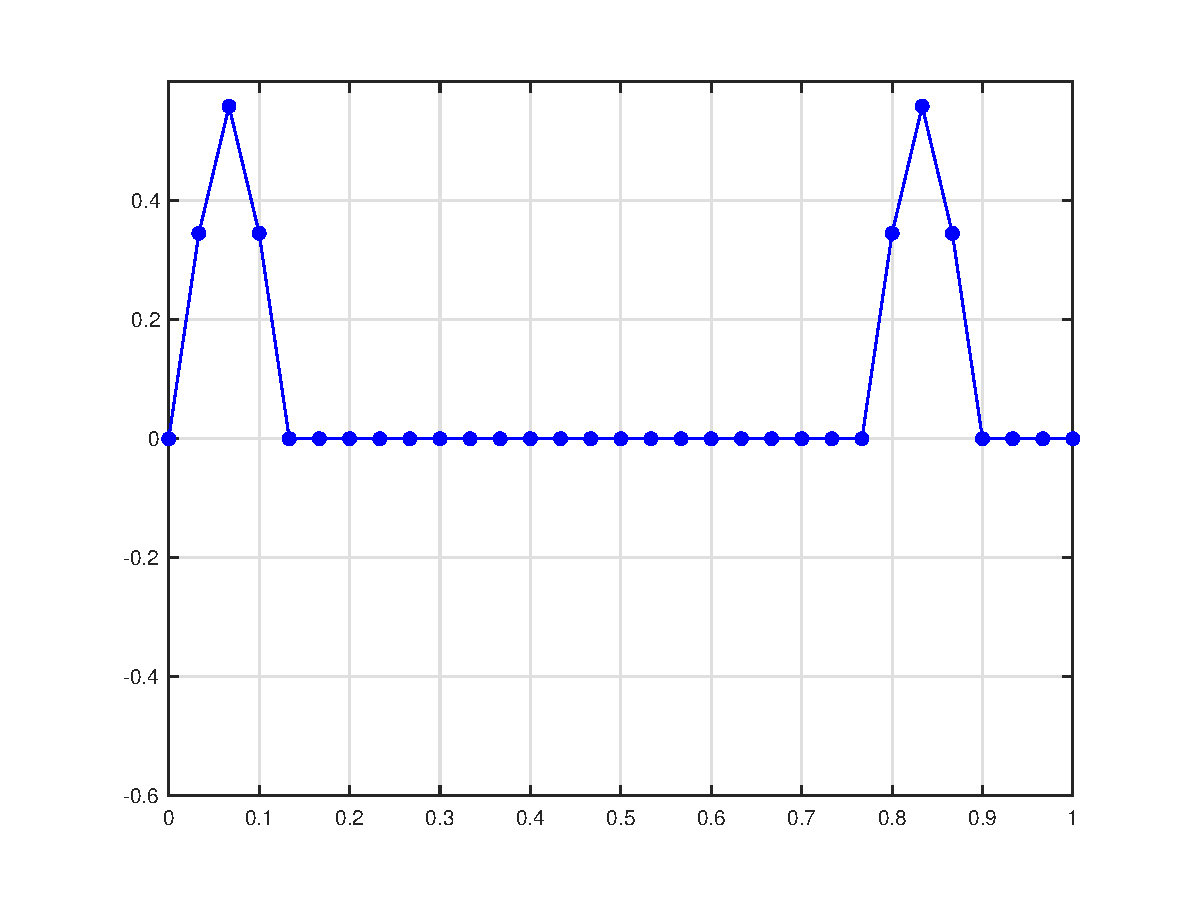
\includegraphics[width=0.6\columnwidth]{plot1.eps}}
% \caption{\label{fig:eta}{String $N=30$.}}
% \end{figure}

Now, imagine detuning the string, or changing the value for tension $T$. If we imagine the tuning knob being at the left boundary, more material will appear on that side when $T$ decreases, and vice versa. To make the transition to the finite-difference setting easier, imagine equidistant points drawn on this string in such a way that there is a point exactly at the nut and the bridge (i.e. at each boundary). Then, when decreasing the tension, the point at the nut (left boundary) will start moving away towards the bridge (right boundary). As a matter of fact, all points (except for the one at the bridge) will start moving towards the bridge! Effectively, we slowly decrease the space between the points which in finite-difference setting is analogous to decreasing the grid spacing according to \eqref{eq:stabilityCondition}. 

The  
% \begin{figure}[h]
% \centerline{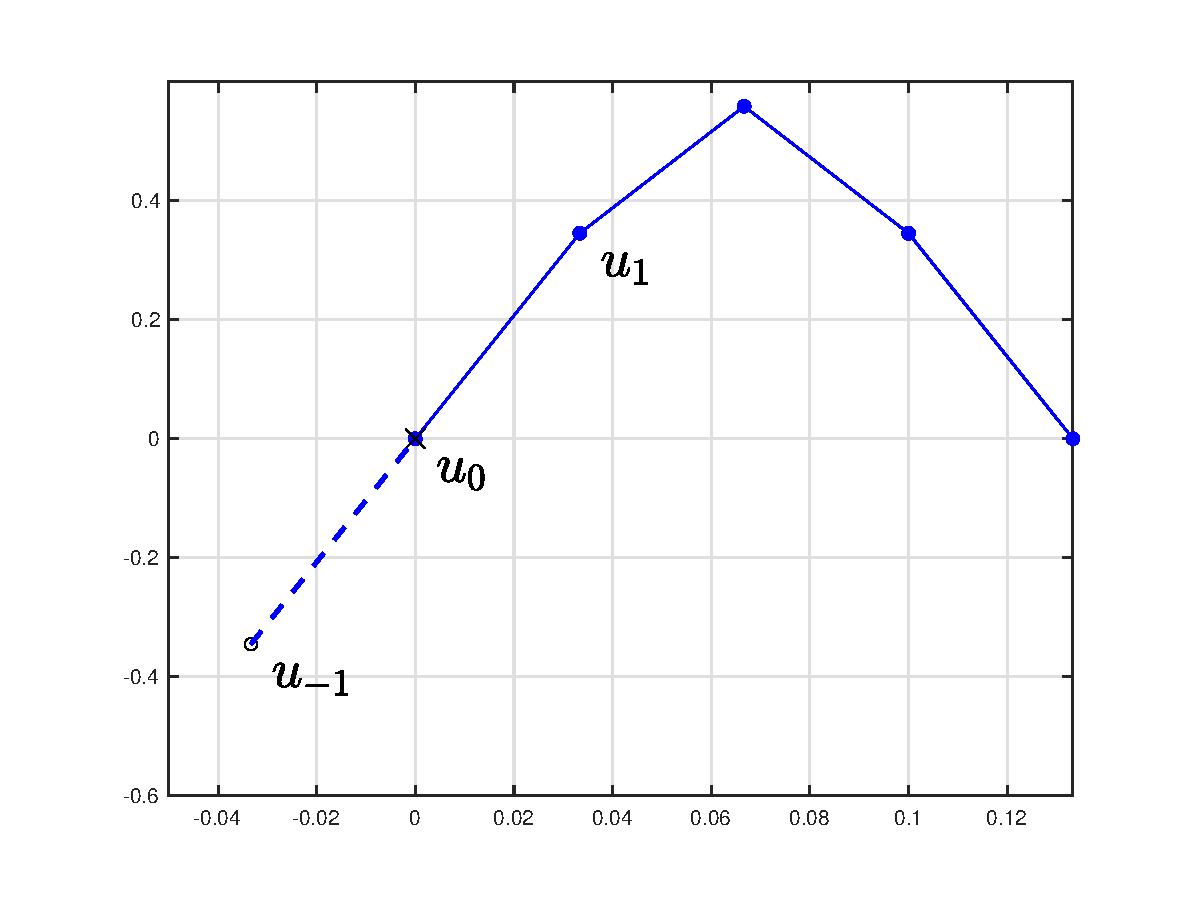
\includegraphics[width=0.6\columnwidth]{plot2.eps}}
% \caption{\label{fig:eta}{At the left boundary.}}
% \end{figure}

% \begin{figure}[h]
% \centerline{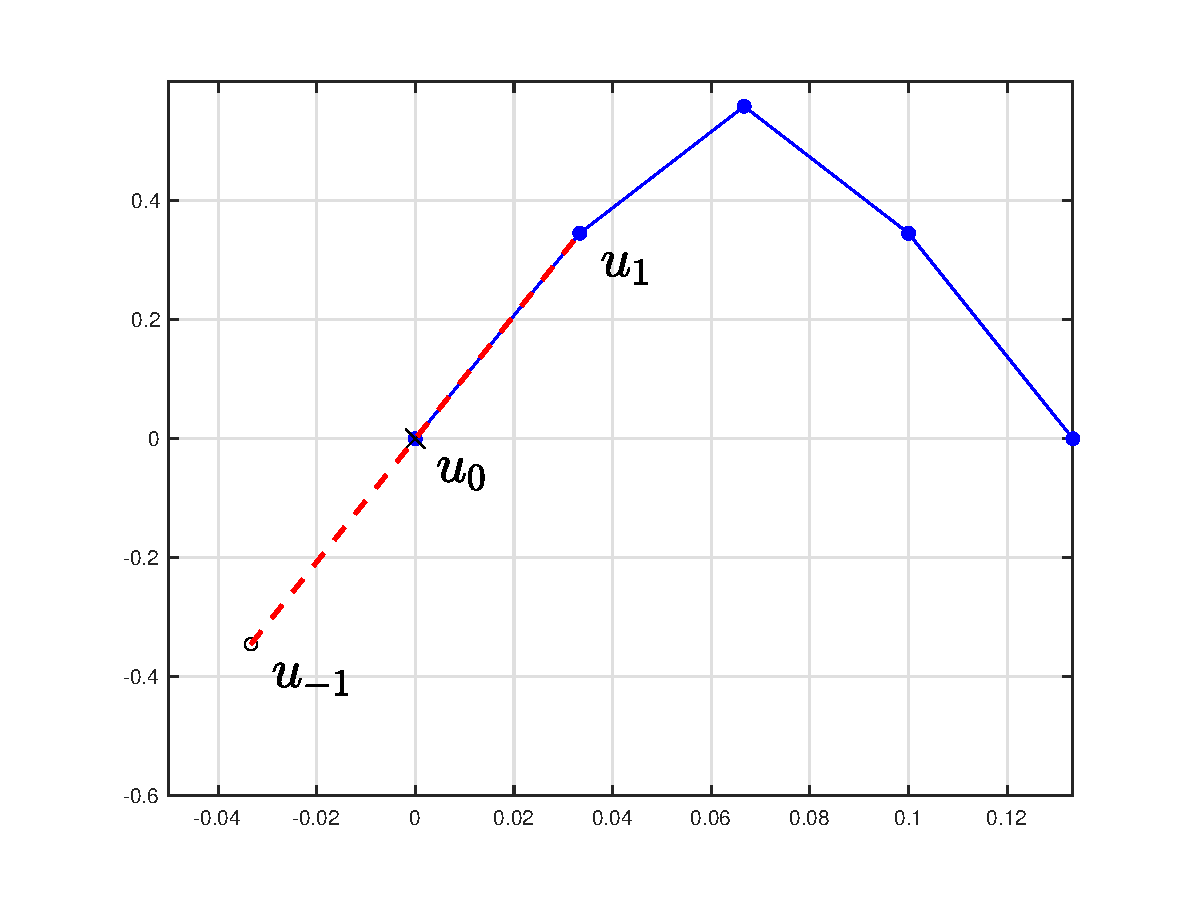
\includegraphics[width=0.6\columnwidth]{plot3.eps}}
% \caption{\label{fig:eta}{Boundary Condition. Curvature at $u_0$ needs to be 0.}}
% \end{figure}

\section{Energy}
We can get the energy of Eq. \eqref{eq:1Dwave} by first taking the inner product with respect to $\delta_{t\cdot}u$ like
\begin{equation}
    \rho A\langle \delta_{t\cdot}u, \delta_{tt}u\rangle_\mathcal{D} - T \langle \delta_{t\cdot}u,\delta_{xx}u\rangle_\mathcal{D} = 0
\end{equation}
using integration by parts to get
\begin{equation}\label{eq:innerProd}
    \rho A\langle \delta_{t\cdot}u, \delta_{tt}u\rangle_\mathcal{D} + T \langle \delta_{t\cdot}\delta_{x+}u,\delta_{x+}u\rangle_{\underline{\mathcal{D}}} = \mathfrak{b}
\end{equation}
where
\begin{equation}
    \mathfrak{b} = T (\delta_{t\cdot}u_N)(\delta_{x+}u_N) - T(\delta_{t\cdot}u_0)(\underbrace{\delta_{x+}u_{-1}}_{\delta_{x-}u_0}).
\end{equation}
Expanding Eq. \eqref{eq:innerProd} yields,
\begin{equation}
    \rho A \sum_\mathcal{D}h(\delta_{t\cdot}u)(\delta_{tt}u) + T \sum_{\underline{\mathcal{D}}}(\delta_{t\cdot}\delta_{x+}u)(\delta_{x+}u)
\end{equation}
Then, we can use the following identities  
\begin{equation}
    (\delta_{t\cdot}u)(\delta_{tt}u) = \delta_{t+}\left(\frac{1}{2}(\delta_{t-}u)^2\right) \quad \text{and} \quad (\delta_{t\cdot}u)u = \delta_{t+}\left(\frac{1}{2}u e_{t-}u\right)
\end{equation}
\end{document}
